\chapter{Introduction to Electricity}

What happens when you turn on a flashlight? The battery in the
flashlight acts as an electron pump, and the electrons flow through the
wires to the lightbulb (or LED). As the electrons pass through the
lightbulb, they excite the molecules within, which gives off light and
heat. (LEDs also give off light and heat, but they give off much less
heat.) The electrons rthen return to the battery to be pumped around
again.

When electricity is flowing through a copper wire, the protons and
neutrons of the copper stay put, while the electrons jump between the
atoms on their way from the battery to the lightbulb and back again.

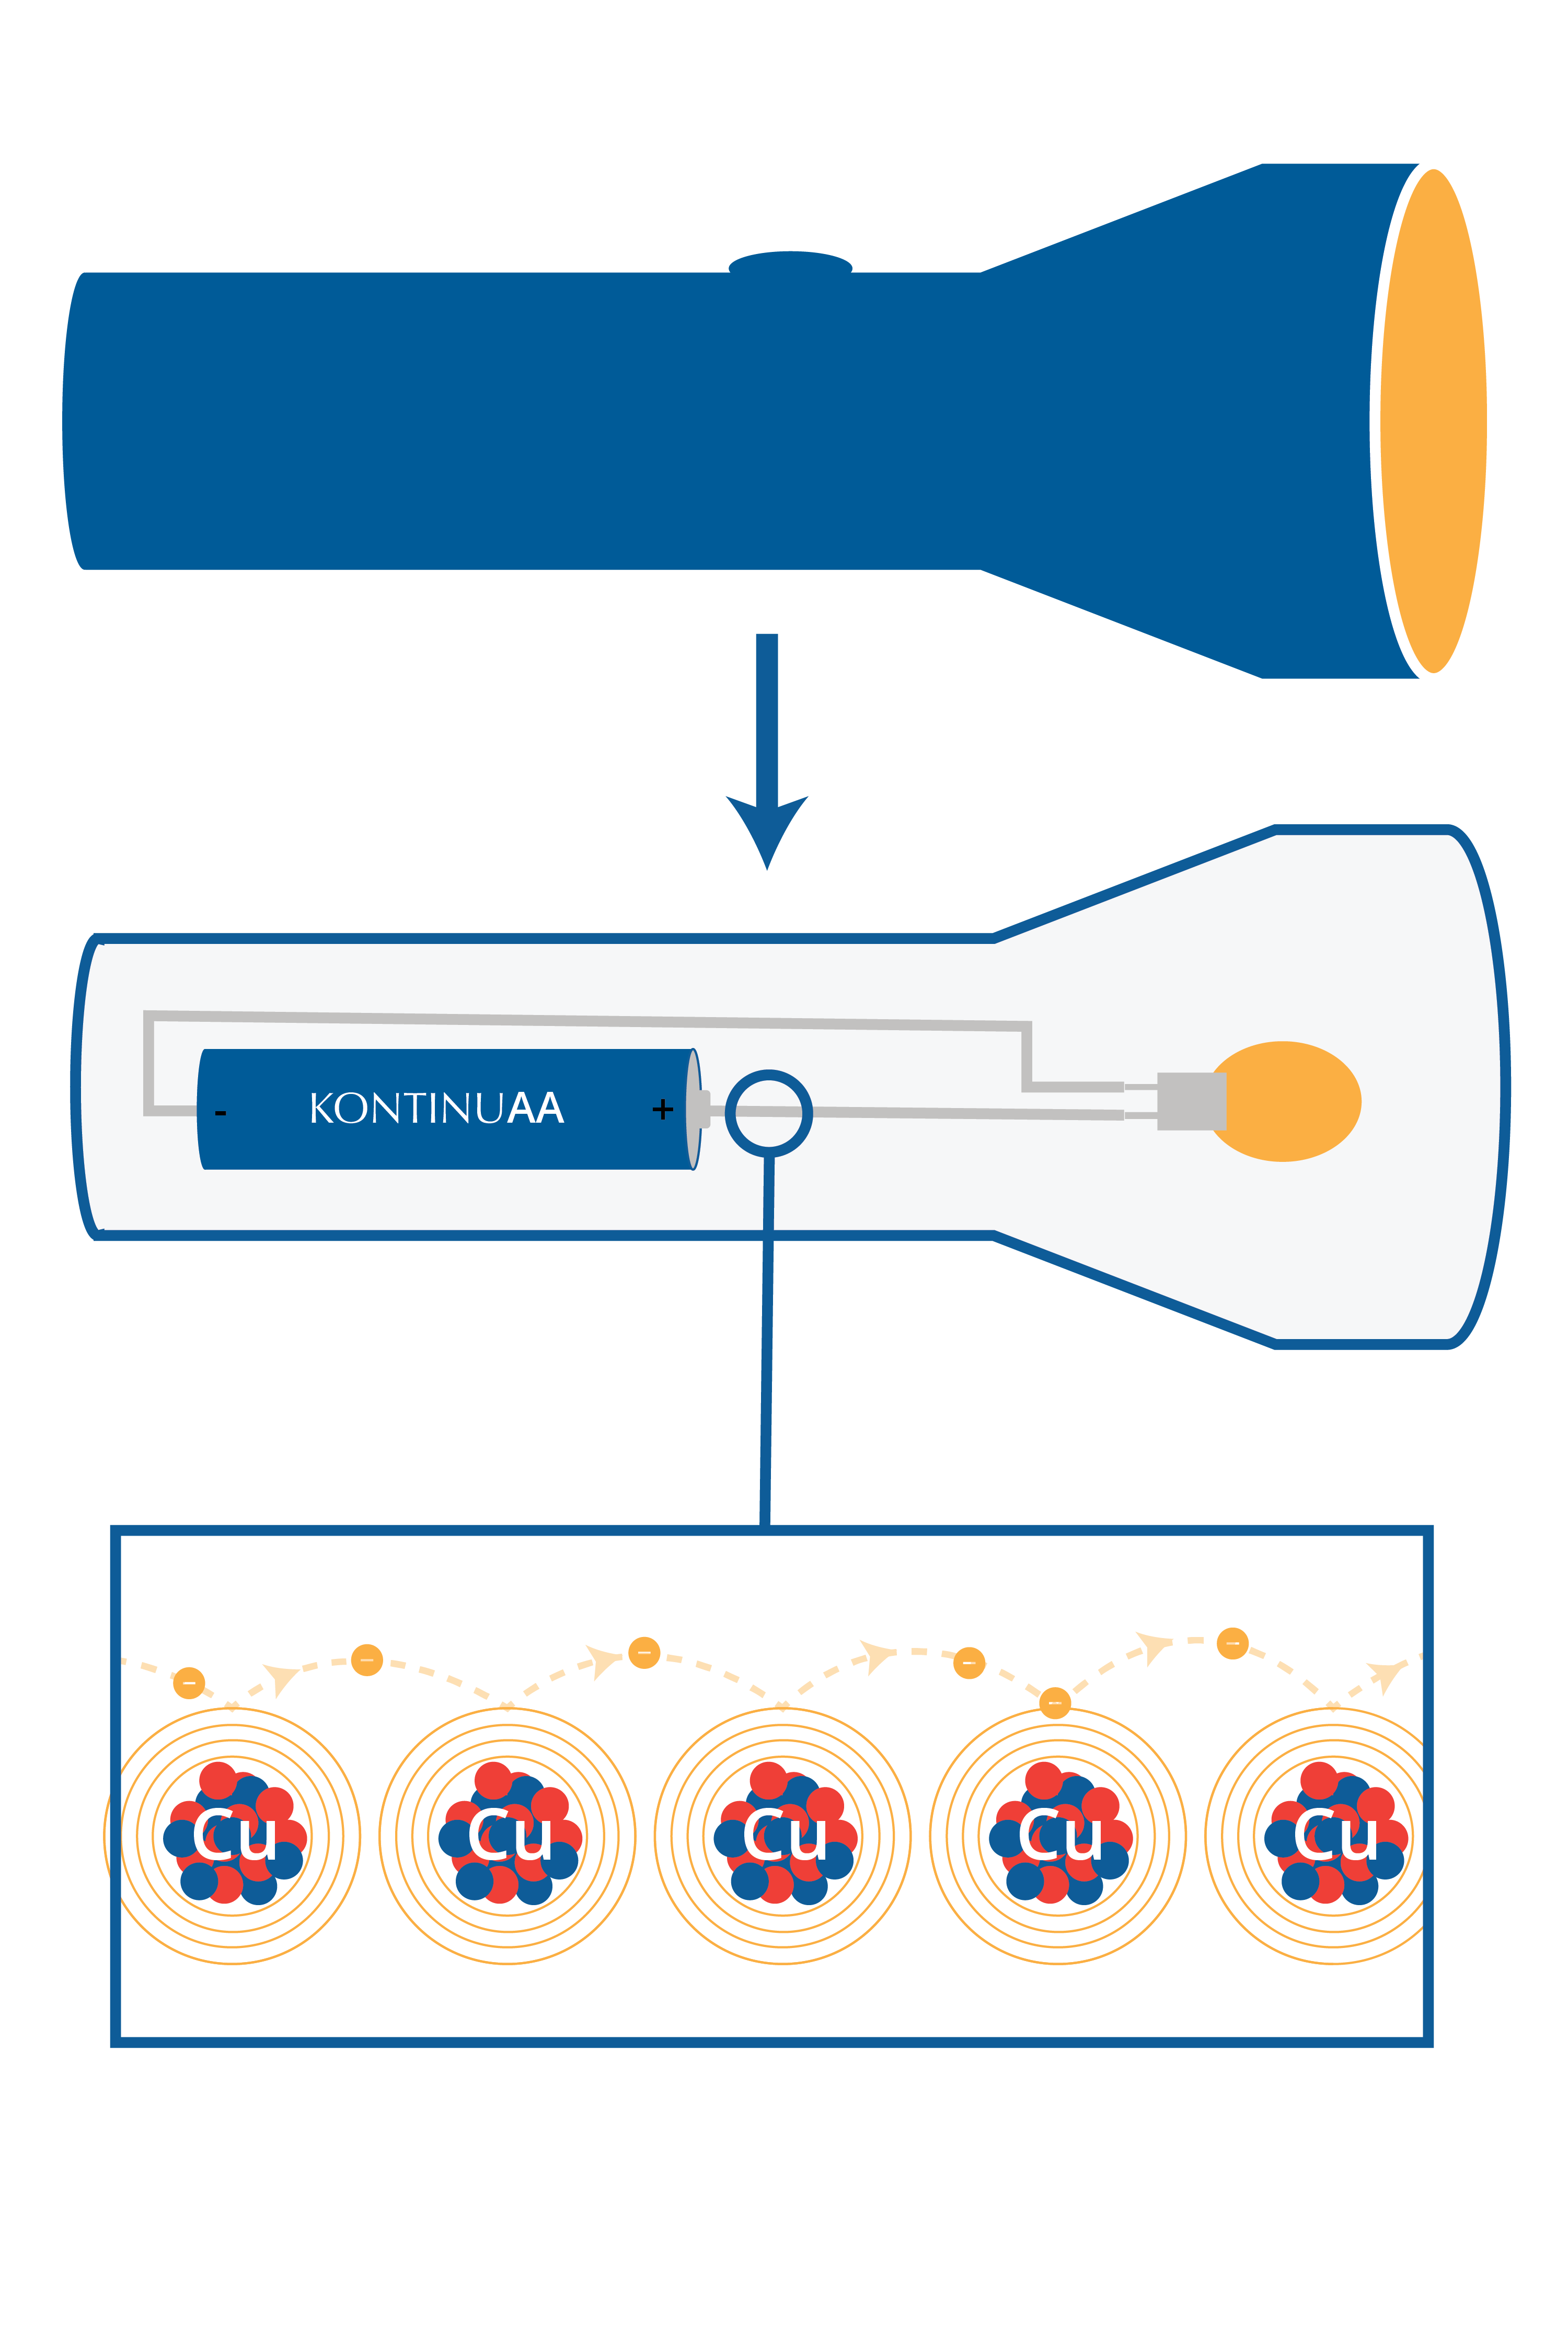
\includegraphics[width=.5\textwidth]{flashlight.png}


In some materials, like copper and iron, electrons are loosely bound
to their nuclei, forming a sea of electrons, which allows energy to flow. These are good \textit{electrical conductors}. In
other materials, like glass and plastic, electrons don't leave their
nuclei as easily. This makes them are terrible electrical conductors -- we call
these materials \textit{electrical insulators}. For example, the plastic around a
wire is used for electrical insulation.

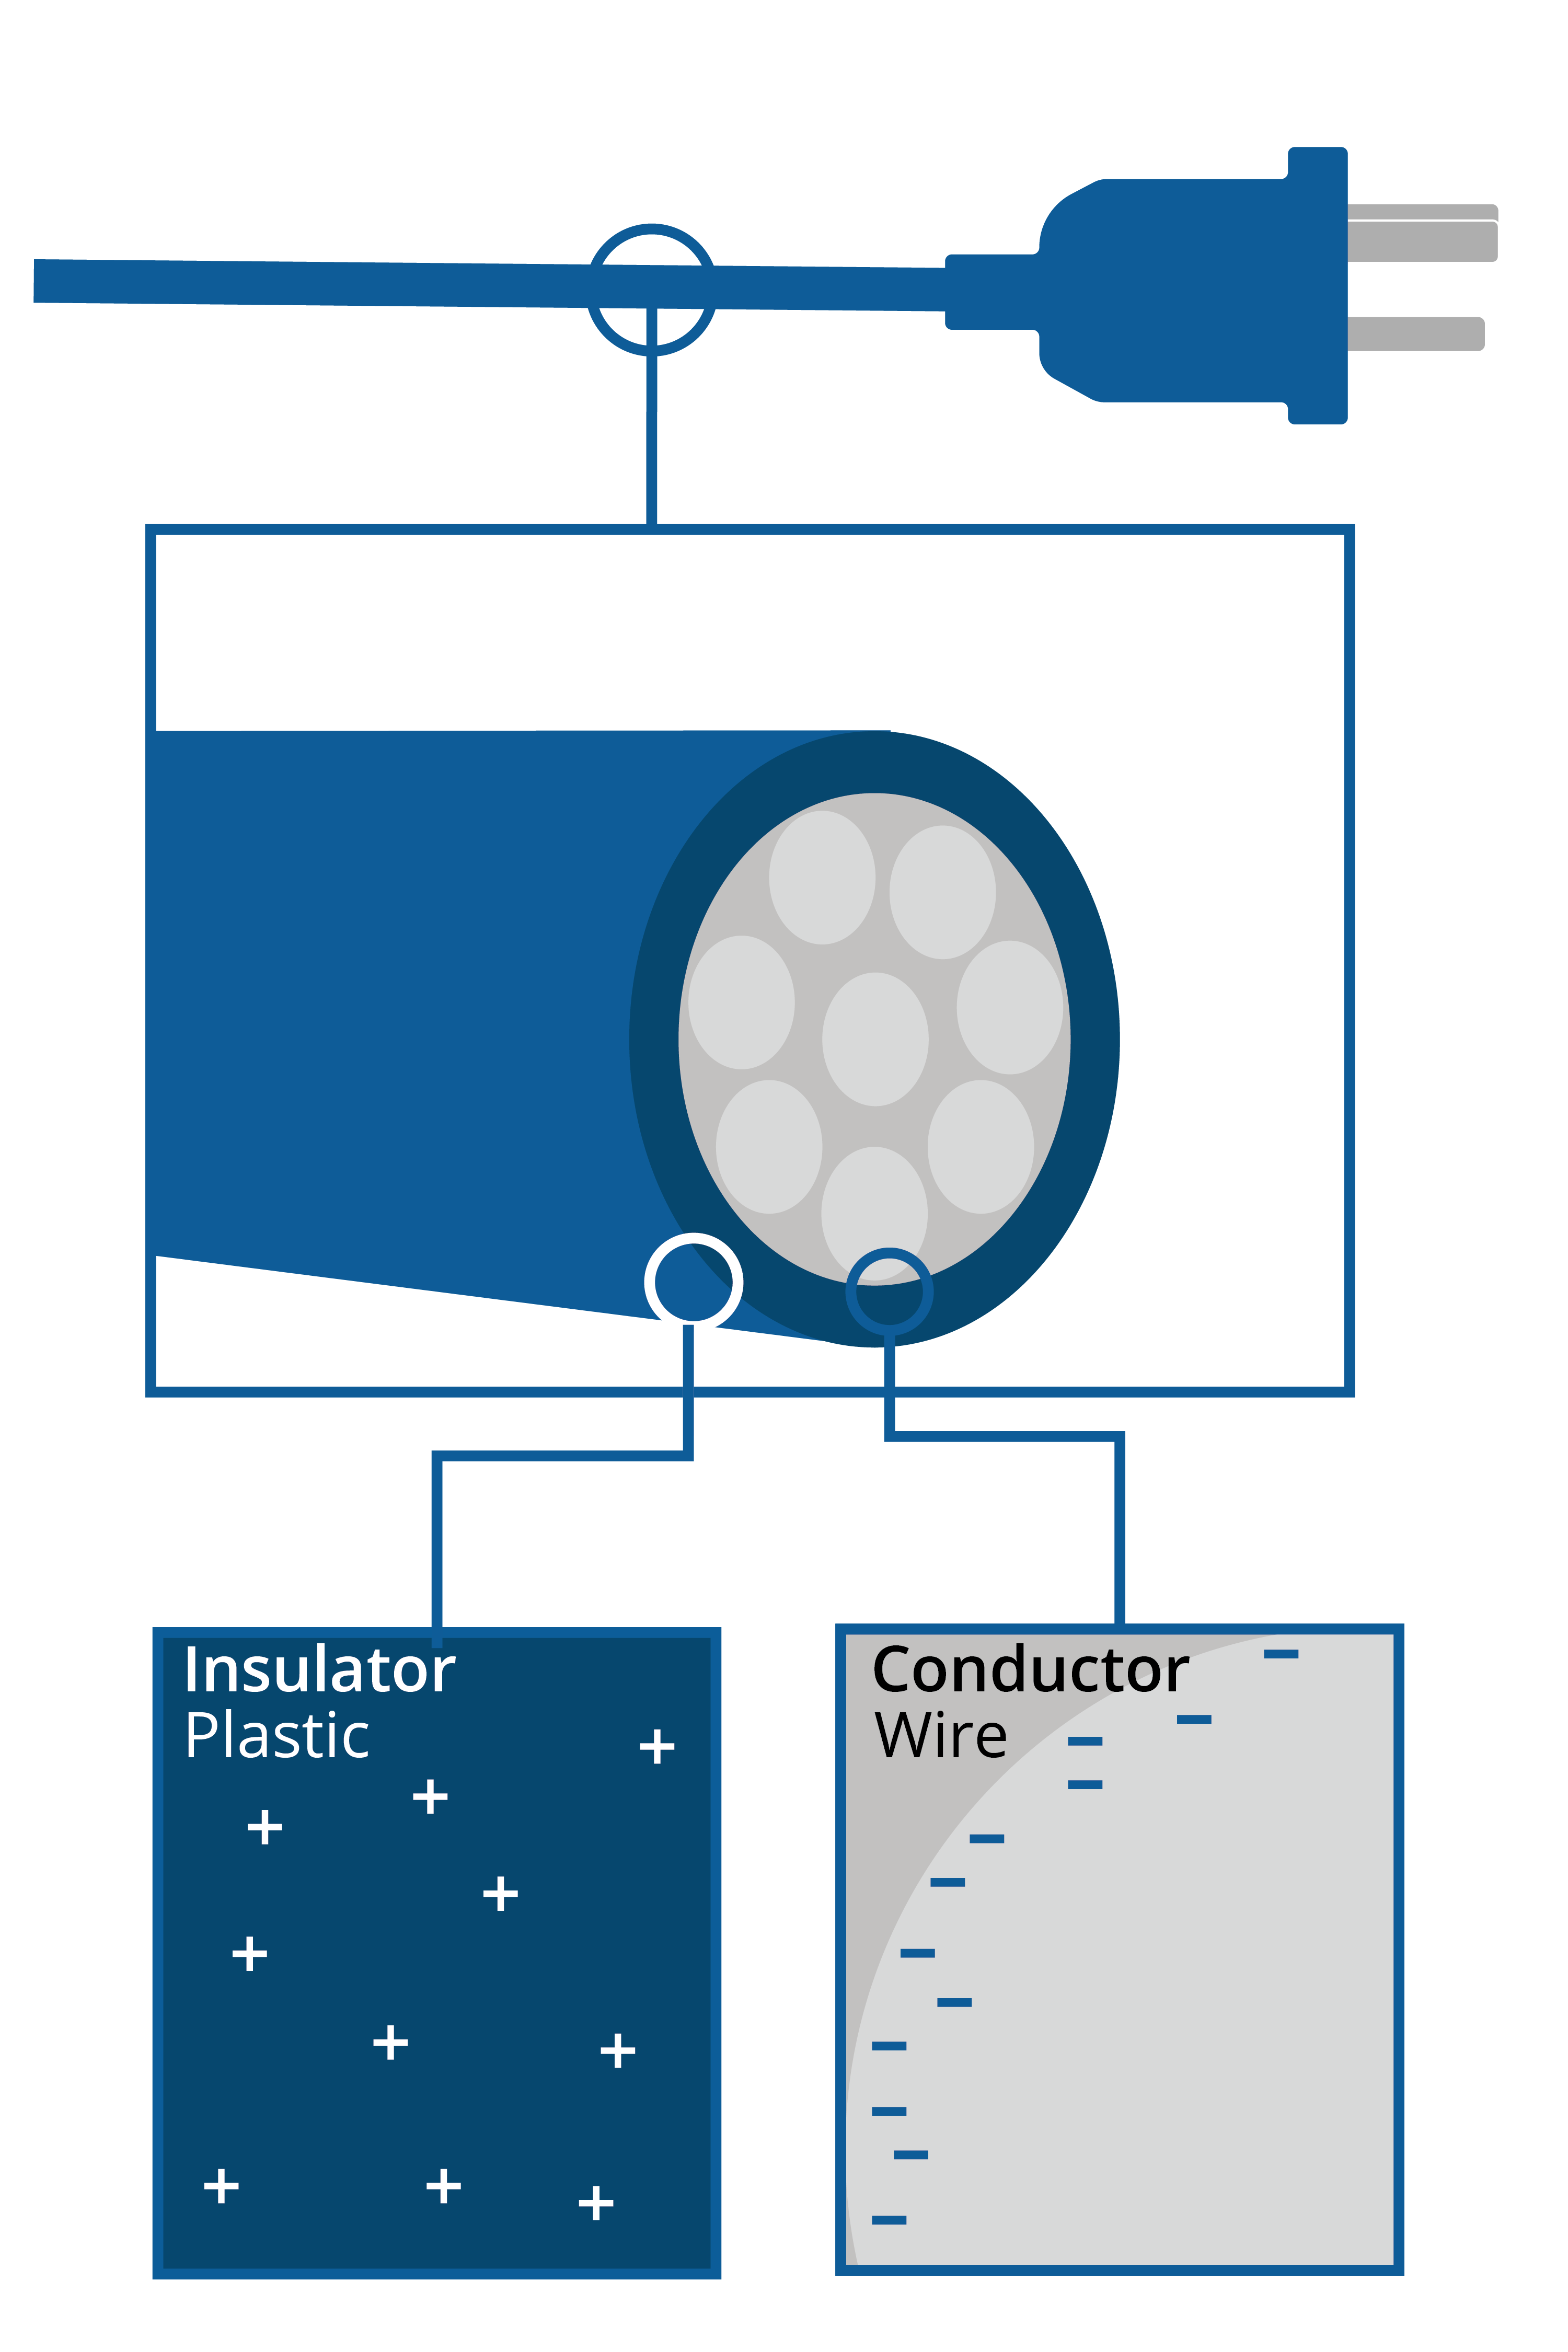
\includegraphics[width=.5\textwidth]{plug.png}

% KA: https://www.khanacademy.org/science/physics/electric-charge-electric-force-and-voltage/charge-electric-force/v/conductors-and-insulators

\section{Units}

Electrons are very small, so to study them, scientists came up with a
unit that represents \textit{a lot} of electrons. 1 \textit{coulomb}
is about 6,241,509,074,460,762,608 electrons. When 5 coulombs enter one end of the wire every second (and simultaneously 5 coulombs exit the other end), we say ``This wire is carrying 5 amperes of current.''\index{coulombs}

(Truthfully, we usually shorten ampere to just ``amp''.  This is
sometimes a little awkward, because we also often shorten the word
``amplifier'' to ``amp,'' but you should generally be able to tell which is which
from the context.)\index{amp or ampere}

If you look at the circuit breakers or fuses for your home's
electrical system, you'll see that each one is rated in amps. For
example, maybe the circuit that supplies power to your kitchen has a 10
amp circuit breaker. If, for some reason, more than 10 amps tries to
pass through that wire, the circuit breaker will turn off the whole
circuit.

When your flashlight is on, it pushes about 1 amp of current
through the lightbulb (When it is off, there is no current in the
lightbulb).

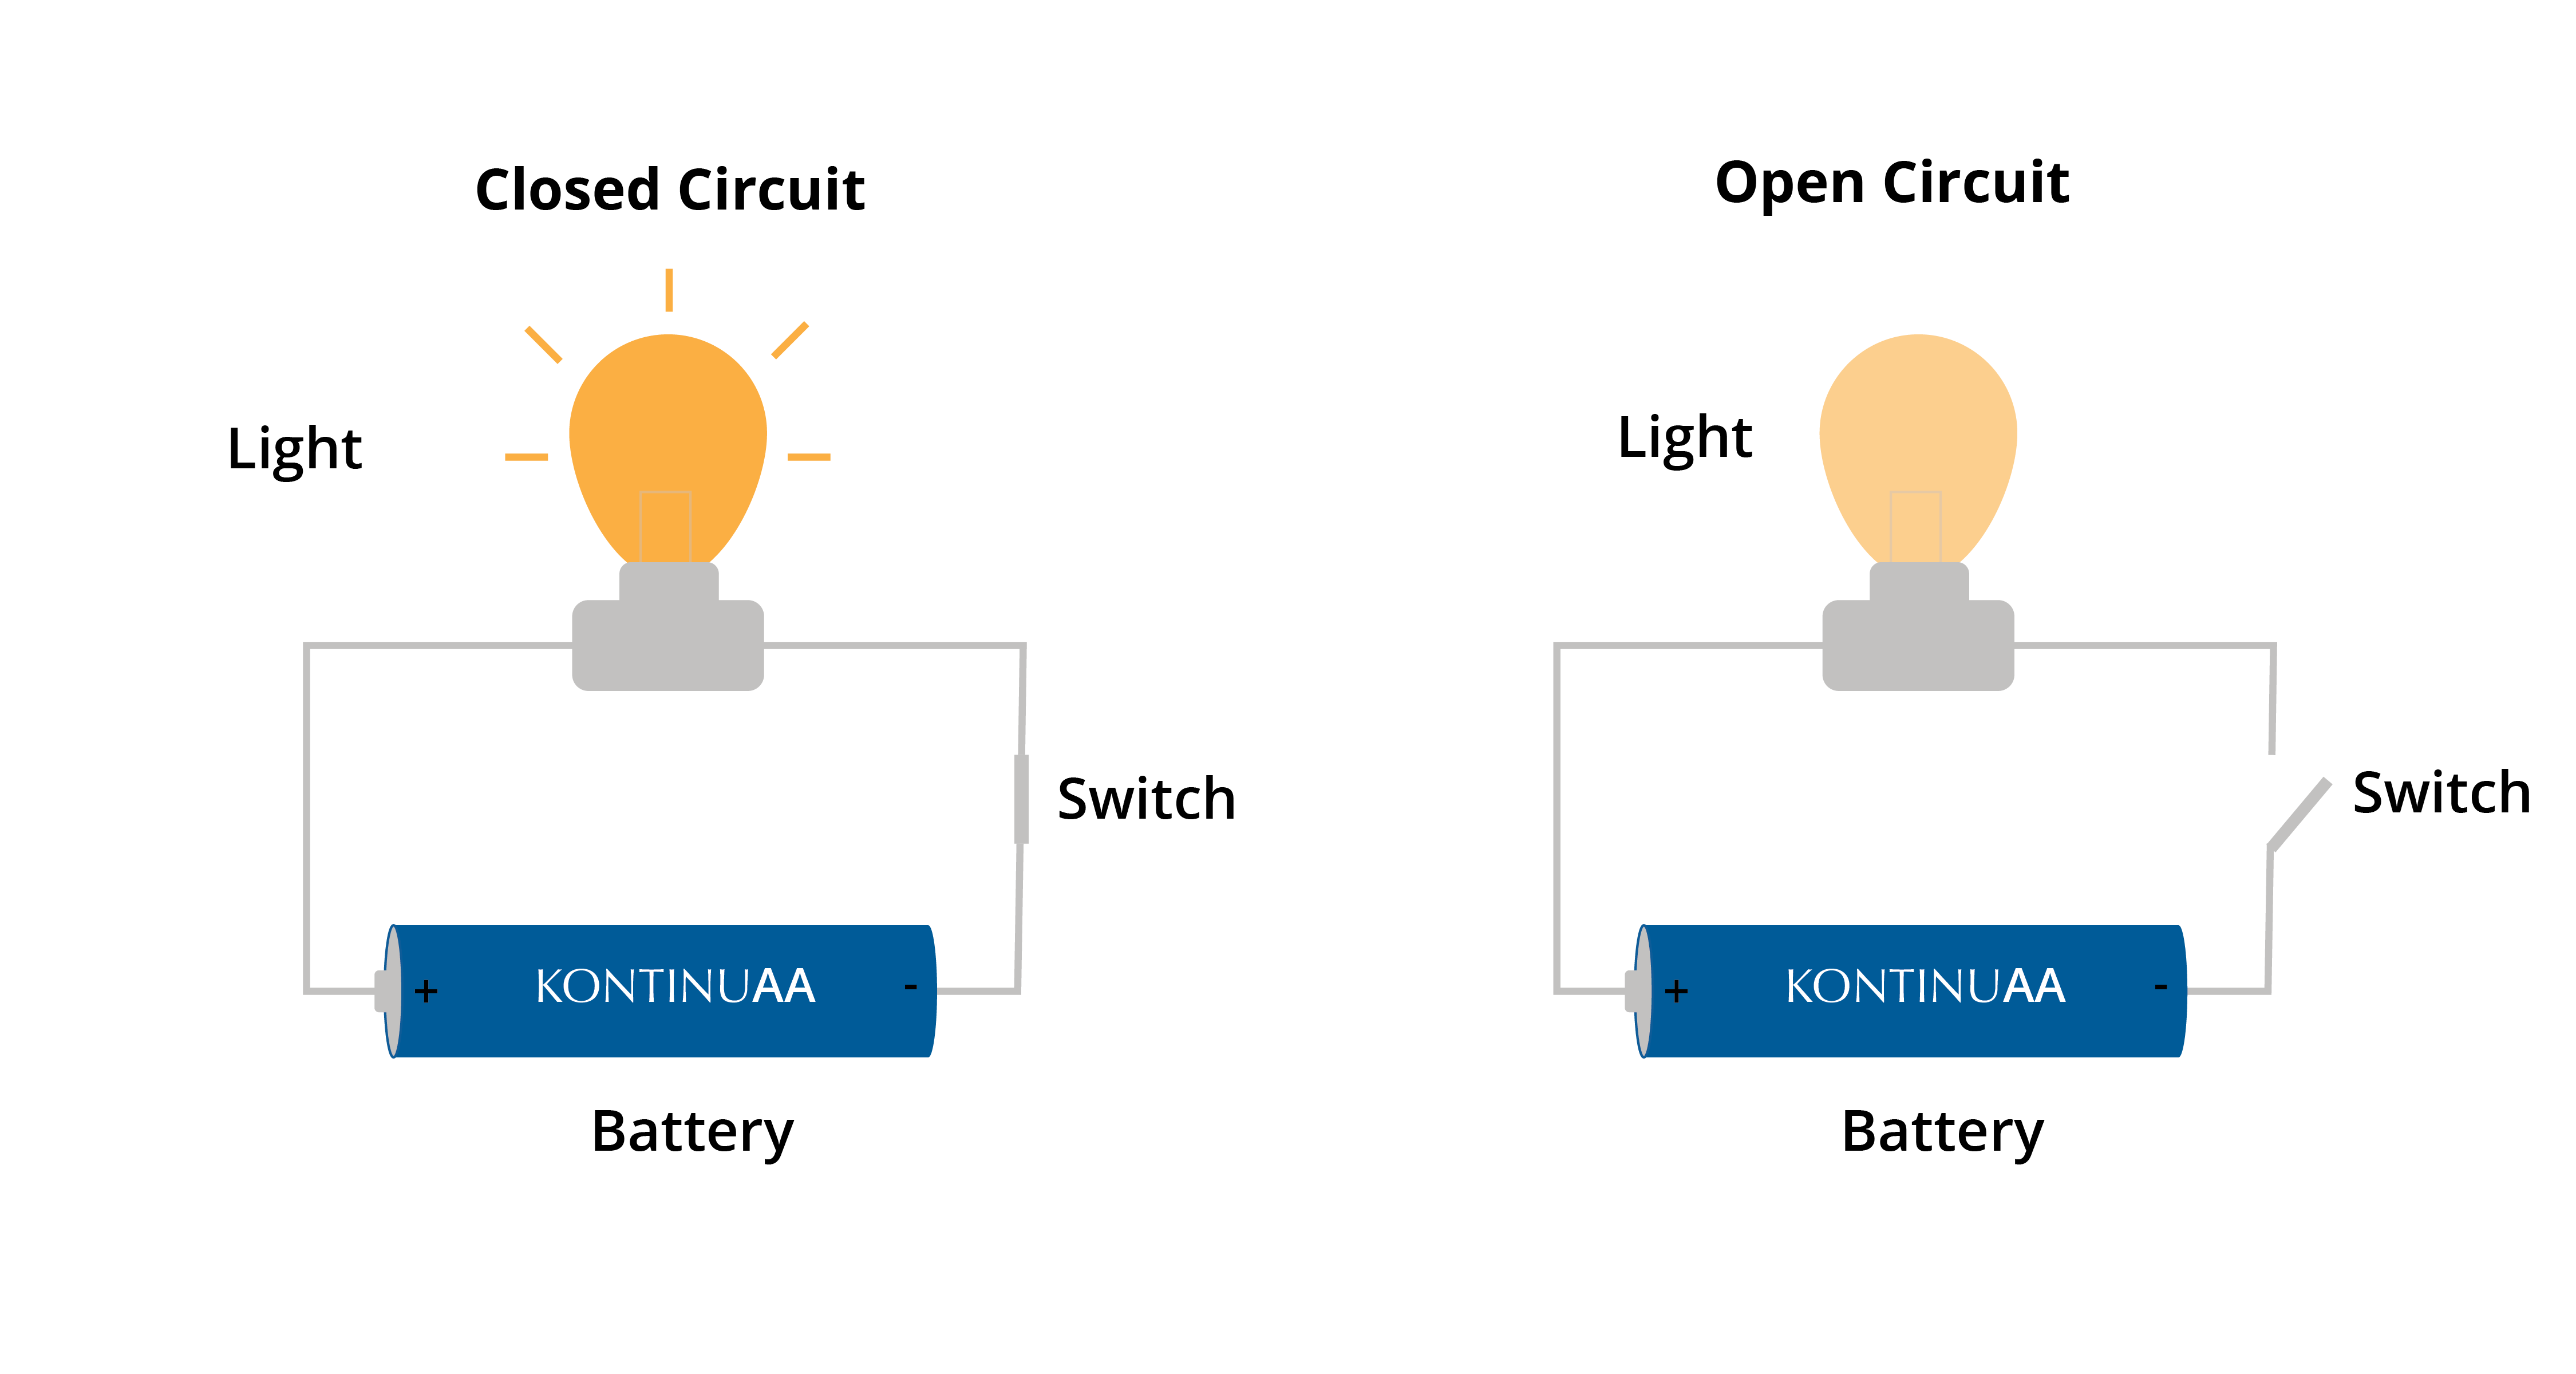
\includegraphics[width=1\textwidth]{Circuit_OnOff.png}

The lightbulb creates \textit{Resistance} that the current pushes
through.\index{resistance} Think of it like plumbing: The current is the amount of water
passing through a pipe. The resistance is something that tries to stop
the current -- like a ball of hair. The battery is what allows
 the current to push through the resistance; we call that
pressure \textit{voltage}.\index{voltage}

\section{Circuit Diagrams}

Here is a circuit diagram of your flashlight:

\begin{circuitikz}
\draw (0,0) to[battery1,invert,l=$3V$] ++(0,3)
to [switch,i=1A] ++(3,0)
to [lamp=$1\Omega$,bipoles/length=0.9cm] ++(0,-3) -- (0,0);
\end{circuitikz}

The lines are wires. The symbols that we will use are:

\begin{tabular}{c c c c}
  Battery & Switch & Lamp & Resistor \\
\begin{circuitikz}
\draw (0,0) to[battery1] (2,0); 
\end{circuitikz}
&
\begin{circuitikz}
\draw (0,0) to[lamp,bipoles/length=0.9cm,l=$3 \Omega$] (2,0); 
\end{circuitikz}
&
\begin{circuitikz}
\draw (0,0) to[switch,/tikz/circuitikz/bipoles/length=1.0cm] (2,0); 
\end{circuitikz}
&
\begin{circuitikz}
\draw (0,0) to[R,  l=$3 \Omega$] (2,0); 
\end{circuitikz} \\
\end{tabular}

The battery pushes the electrons from one end and pulls them back in at the other, so the circuit must go around in a circle for the current to flow. This is why the current stops flowing when the switch breaks the circuit.

You can think of a switch as having zero resistance when it is closed and infinite resistance when it is open.


For our purposes, a lamp is just a resistor that gives off light.
% KA: https://www.khanacademy.org/science/high-school-physics/dc-circuits/electric-power-and-dc-circuits/a/circuit-introduction

\section{Ohm's Law}

Resistance is measured in \textit{ohms}, and we use a Greek capital omega for that: $\Omega$  

Voltage is measured in
\textit{volts}.\index{ohms}\index{volts}

\begin{mdframed}[style=important, frametitle={Ohm's Law}]\index{Ohm's law}
  Whenever a voltage $V$ is pushing a current $I$ through a resistance of $I$, the following is true:

  $$V = IR$$

  where $V$ is in volts, $I$ is in amps, and $R$ is in ohms.
\end{mdframed}
% KA: https://www.khanacademy.org/science/physics/circuits-topic/circuits-resistance/v/circuits-part-1

\section{Power and Watts}

\begin{mdframed}[style=important, frametitle={Joule's Law}]\index{Joule's law}

  When a current $I$ is passing through a resistance $R$, the power consumed is
  
  $$W = I^2 R$$

  where $W$ is in watts, $I$ is in amps, and $R$ is in ohms.
\end{mdframed}

Of course $V = IR$, so we can extend this to:

$$W = I^2 R = I V = \frac{V^2}{R}$$

Your flashlight's batteries provide about 3 volts. How much
battery power is the flashlight using when it is on? The power (in
watts) produced by the battery is the product of the voltage (in
volts) and the current (in amps). This means your flashlight is giving off $3
volts \times 1 amp = 3 watts$ of power. Some of that power is given
off as light, some as heat.\index{watts}

A watt is 1 joule of energy per second. We say that a watt is a
measure of \textit{power}.

When we talk about how much energy is stored in a battery, we use a
unit like a kilowatt-hour. A kilowatt-hour is equivalent to 3.6 million
joules.

\section{Another great use of RMS}

In many electrical problems, the voltage fluctuates a great deal.  For
example, the fluctuations in voltage makes the sound that comes out of an
audio speaker.

You can use the root-mean-squared of the voltage to figure out the average power
your speaker is consuming.

Let's say that the RMS of the voltage you are sending to the speaker is $V_{rms}$
and the resistance of the speaker is $R$ ohms. This means the power consumed
by the speaker is:

$$P = \frac{V_{rms}^2}{R}$$

Similarly, if you know the RMS of the current you are pushing through
the speaker is $I_{rms}$, then the power consumed by the speaker is:

$$P = I_{rms} R$$

\section{Electricity Dangers}

Large amounts of electricity moving through your body can hurt or even kill
you. You must be careful around electricity.

That said, your body is not a very good conductor, so low-voltage
systems (like a flashlight) don't have enough voltage to move significant amounts of
current through your body.

However, the  electricity in a power outlet has much more voltage. The voltage
in these outlets is fluctuating between positive and negative, so we
call it \textit{Alternating Current} or AC.
% ADD: Introduce difference between AC and dc

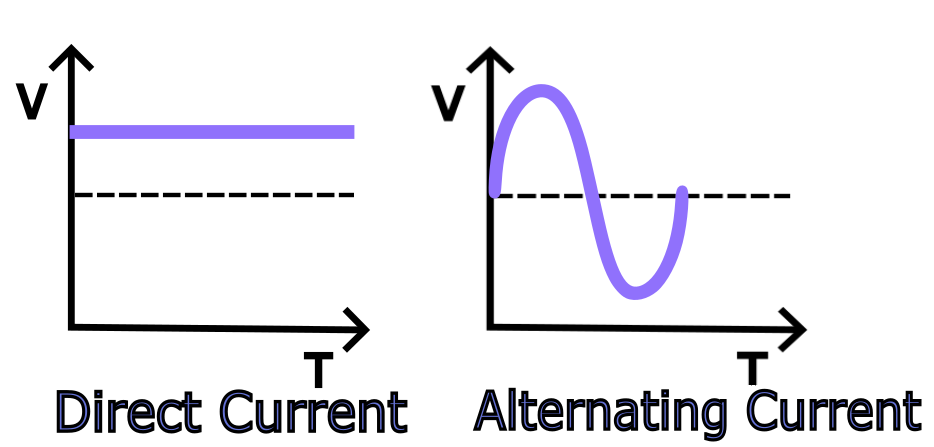
\includegraphics[width=.75\textwidth]{AC_vs_DC.png}

In most countries, the RMS of the voltage between 110 and 240 V. (The
peak voltage is always $\sqrt{2}$ times the RMS value. In the US, for
example, people say ``Our outlets supply 120 V.'' They mean that the
RMS of the voltage difference between the wire and the earth is 120V.
The peak voltage is almost 170V.)

How much current can a human handle? Not much. You can barely feel 1
mA moving through your body, but at 16 mA, your muscles will clench
and you won't be able to relax them --- many people die from
electrocution because they grab a wire which pushes enough current
through their body to prevent them from letting go of the wire. At 20
mA, a human's respiratory muscles become paralyzed.

The fuse breaker in a house will often allow 20 A to flow through the
circuit before it shuts off the power. Always be very sure to shut off
the power before touching any of the wiring in your house.

While water is actually a mediocre conductor, it can still deliver enough current
to kill you. If you see a wire in a puddle, you should not touch the
puddle. Interestingly, because of the salt, sea water is more than
100 times better at conducting electricity than the water you drink.
% ADD: Sea of electrons makes a good conductor

% 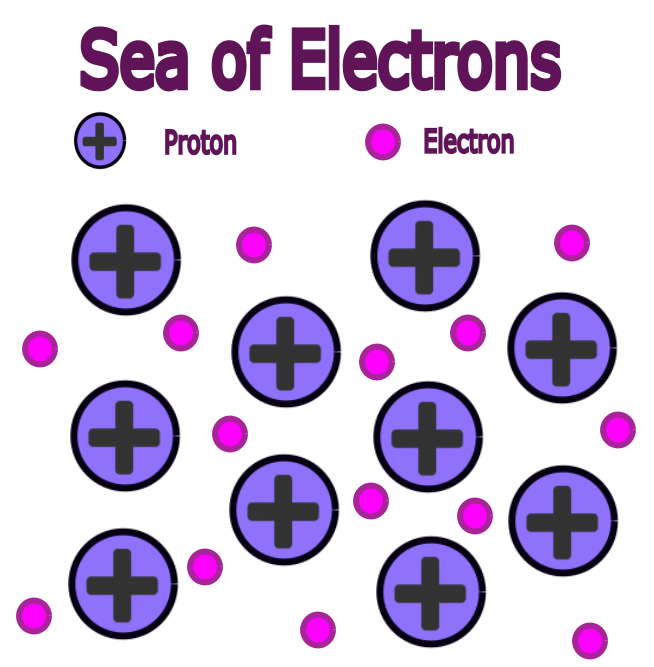
\includegraphics[width=0.8\textwidth]{Sea_Electrons.png}

If you hold a wire in each hand, how many Ohms of resistance will your
body have? Once it gets past your skin, you will look like a bag of
salt water to the electricity. After the skin, your body will have a
resistance of about 300$\Omega$. However, the skin is a pretty good
insulator. If you have dry, calloused hands, your skin may add
100,000$\Omega$ to the resistance.

% KA: https://www.khanacademy.org/science/in-in-class10th-physics/in-in-electricity/in-in-electric-power-and-heating-effect-of-current/v/electric-power-energy

